\clearpage
\section{Deployment case study: policy freshness and observed-event coverage}
\label{app:jetstream}
We deployed a research harness on Jetstream with separate business and audit
PostgreSQL instances, a private report service, and Qdrant retrieval. Raw records
and model prompts remain on the business side. These experiments exercise the
reporting and authorization substrate, not the semantic detectors evaluated
above. A signature authenticates an issuer's claim, not its truth or completeness.

\begin{figure}[ht]
\centering
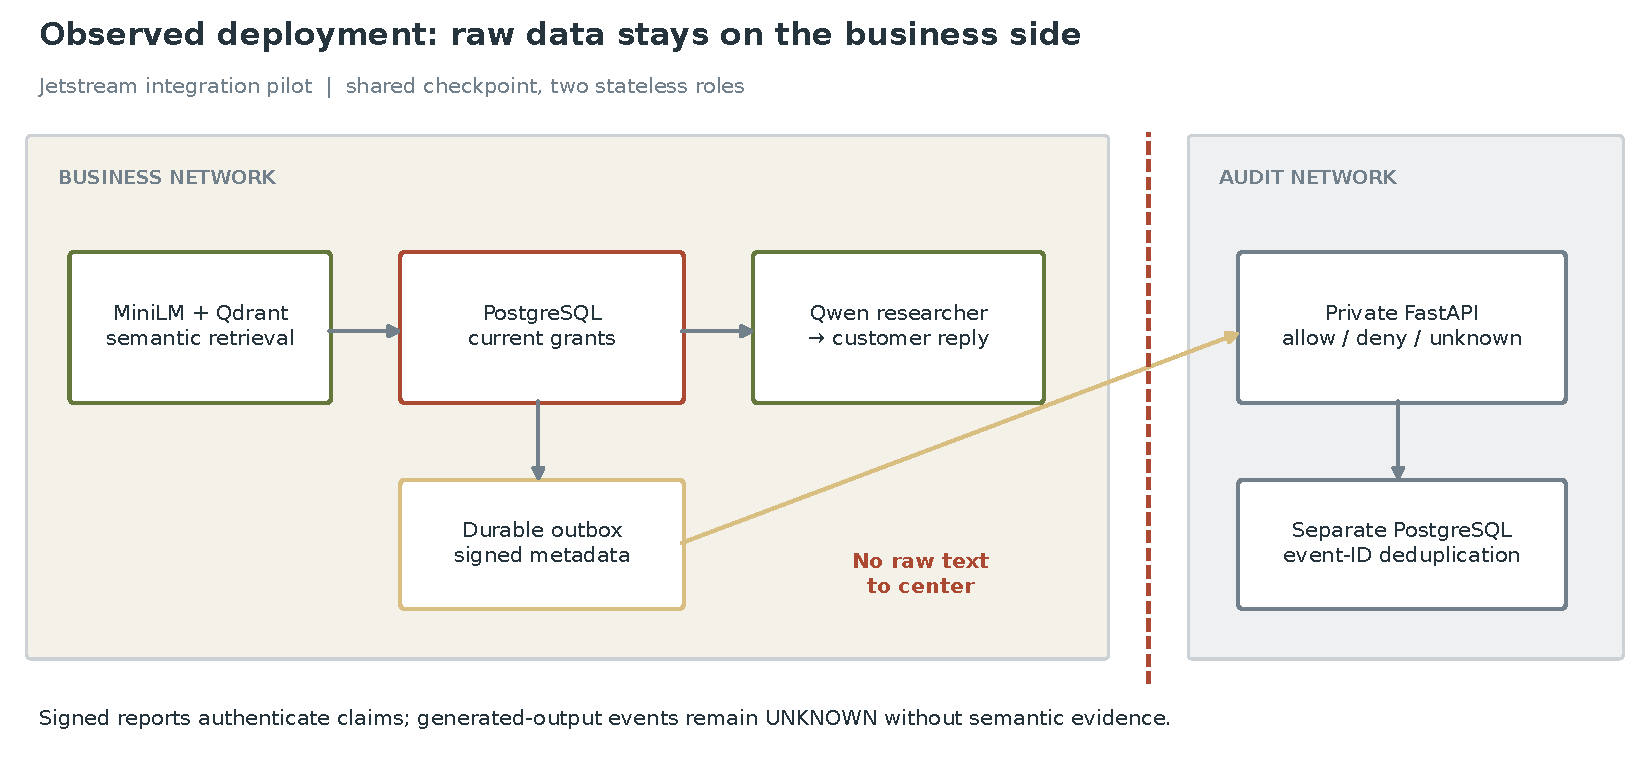
\includegraphics[width=\linewidth]{figures/jetstream20261013/01_deployment.pdf}
\caption{Deployed research pipeline. Missing semantic evidence is reported as
unknown rather than treated as a successful audit.}
\label{fig:jetstream-deploy}
\end{figure}

A controlled regression executed 1,872 operations over 2, 8, and 16 logical tenants,
concurrency levels 1 and 4, three repetitions, six authored scenarios, and two
strategies. These are repeated conditions, not independent semantic examples.
In the constructed revoke and delete cases, a retrieval-time permission snapshot
admitted all 156 operations per case; a delivery-time recheck admitted none.
The recheck failed closed for all 156 otherwise authorized operations with injected
policy unavailability. A subsequent schema revision transported explicit unknowns:
all 48 new regression event IDs reached the center, including 26 unknowns.
A real report-service outage preserved committed outbox records for explicitly
triggered recovery. These observations expose an availability tradeoff, rather
than establishing population-level privacy effectiveness.

\clearpage
\begin{figure}[ht]
\centering
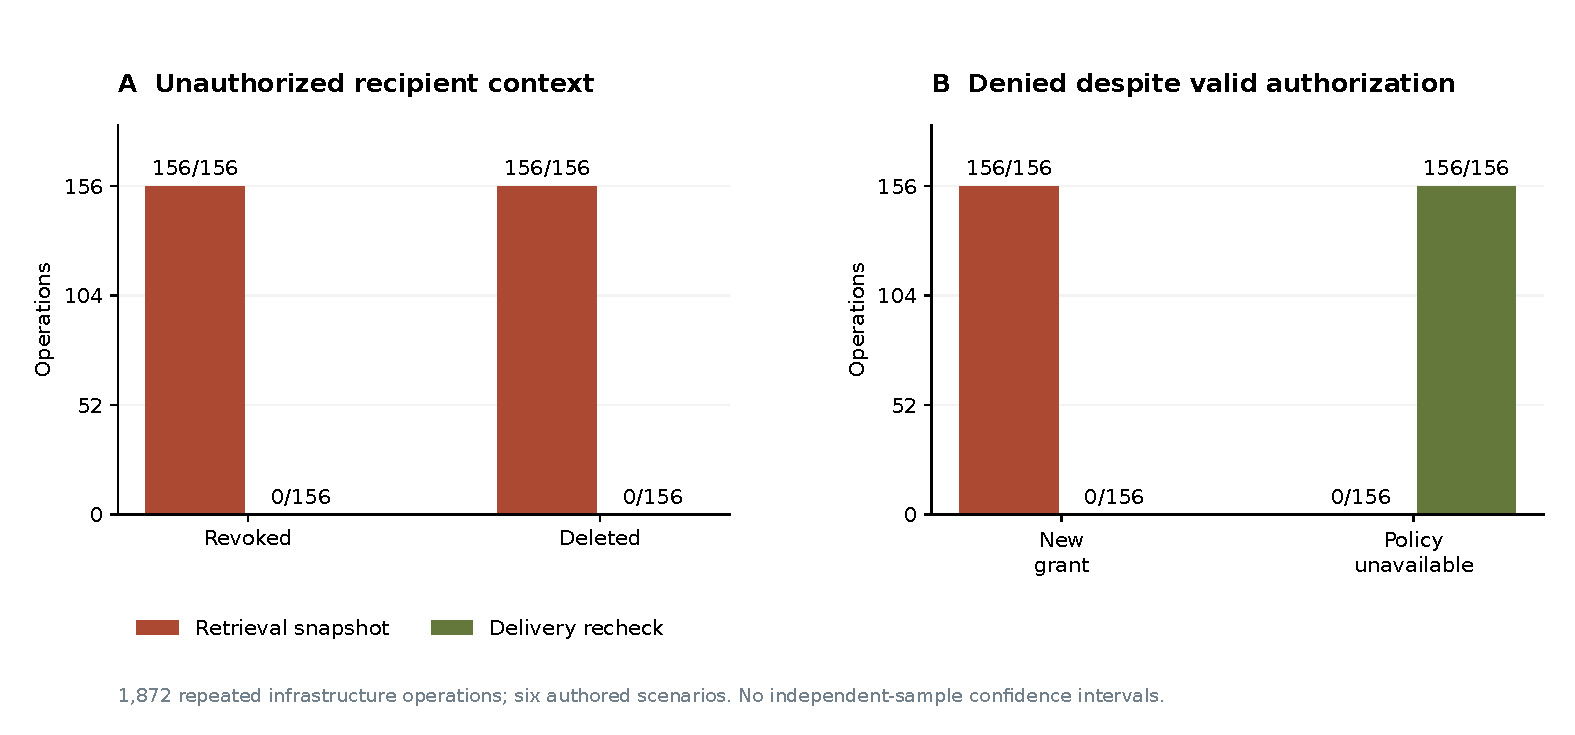
\includegraphics[width=\linewidth]{figures/jetstream20261013/02_policy_tradeoff.pdf}
\caption{Permission freshness regression. Counts reflect authored mutations.
Policy unavailability is injected; the separate report-service outage test
uses an actual stopped container.}
\label{fig:jetstream-policy}
\end{figure}

\paragraph{Online two-role pilot.}
A separate LangGraph pilot used MiniLM embeddings over six synthetic records and
two stateless Qwen2.5-3B-Instruct roles. Four tasks and two controls yielded eight
episodes and 16 generations. All 40 observed event IDs reached the center,
including 16 generated-output observations marked unknown. This does not detect
unreported events. A snapshot-controlled episode propagated a revoked identifier
into its handoff and final answer; the paired recheck withheld that record.
Nevertheless, the recheck answer misattributed another customer's tracking
reference. Required-term presence therefore does not establish task success.

Twelve of 16 generations reached the 96-token cap. We preserve these results and
do not use the pilot to estimate semantic audit recall or general task success.
Independent human semantic review has not been completed. These observations
establish a working research harness, not production readiness.

\clearpage
\begin{figure}[ht]
\centering
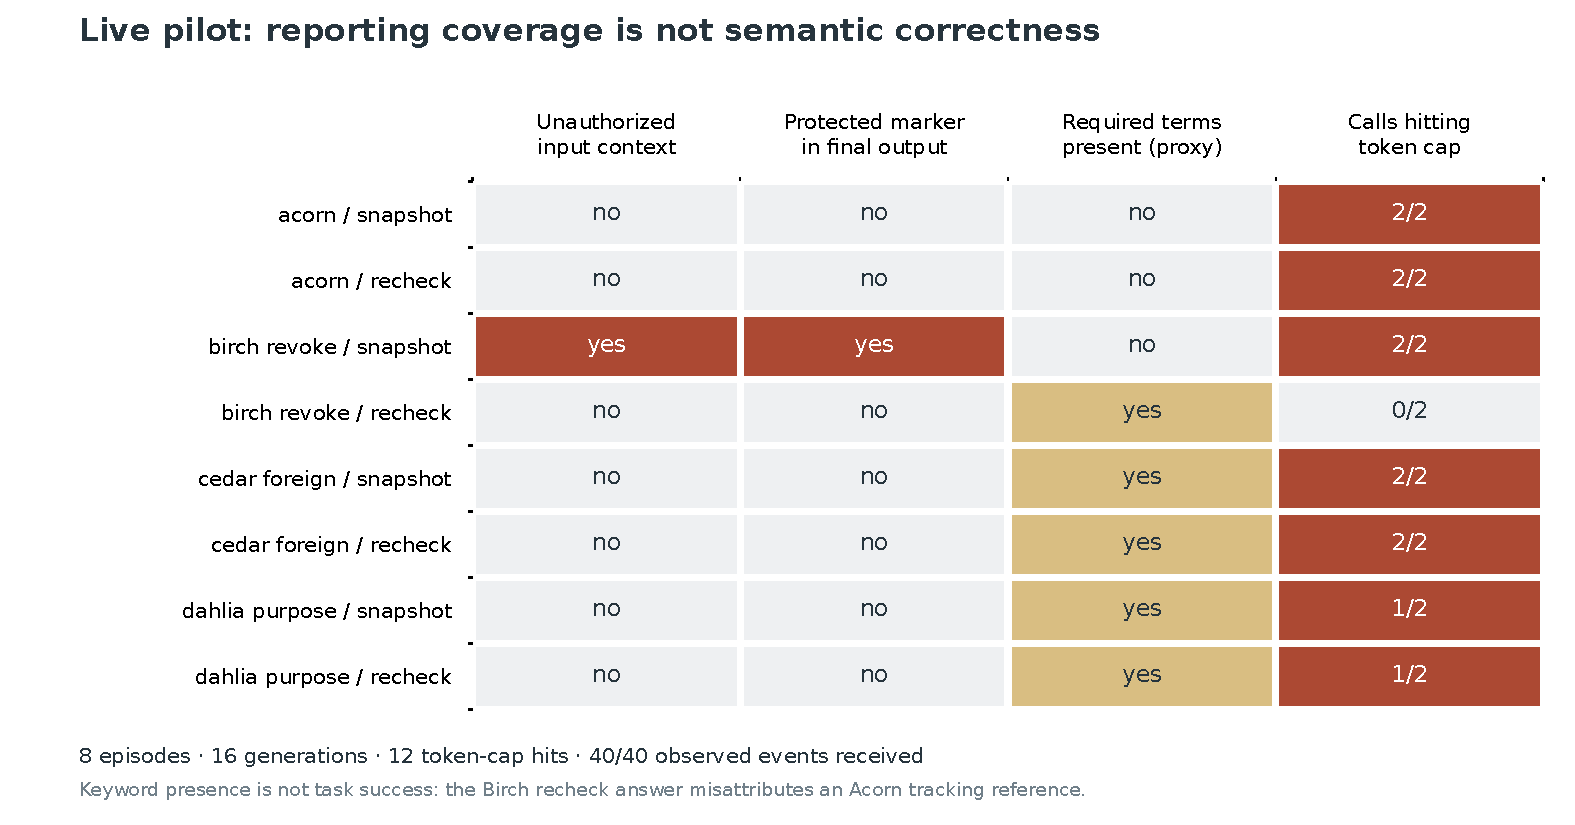
\includegraphics[width=\linewidth]{figures/jetstream20261013/03_live_limitations.pdf}
\caption{Pilot outcomes. Keyword presence is an automatic proxy, not a semantic
judgment. Raw responses expose misattribution despite a positive proxy.}
\label{fig:jetstream-limitations}
\end{figure}
\clearpage

\paragraph{Development follow-up: retrieval scope and policy freshness.}
A second frozen run reused the four development tasks with four configurations:
broad or case-scoped retrieval crossed with snapshot or delivery-time checks.
All 16 episodes and 32 generations completed without execution errors or token-cap
hits. Both snapshot configurations exposed the revoked Birch reference, whereas
both recheck configurations withheld it. The broad recheck answer nevertheless
substituted Acorn's reference. The scoped recheck answer avoided that substitution
but asserted that the refund had not been processed, unsupported by its available
records. These observations motivate Section~\ref{sec:methodology}; they are not
independent human semantic judgments. The prompt and output cap changed from the
first pilot (96 to 256 tokens), so differences across pilots do not isolate the
effect of retrieval scope. Raw traces, frozen protocol, model manifest, and
unfilled human-review forms are preserved under
\texttt{deploy/research/results/live-v2-20261013/}.
